% !TEX encoding = UTF-8 Unicode
\documentclass[a4paper]{article}

\usepackage{color}
\usepackage{url}
\usepackage[T2A]{fontenc} % enable Cyrillic fonts
\usepackage[utf8]{inputenc} % make weird characters work
\usepackage{graphicx}

\usepackage[english,serbian]{babel}
%\usepackage[english,serbianc]{babel} %ukljuciti babel sa ovim opcijama, umesto gornjim, ukoliko se koristi cirilica

\usepackage[unicode]{hyperref}
\hypersetup{colorlinks,citecolor=green,filecolor=green,linkcolor=blue,urlcolor=blue}

\usepackage{listings}
\usepackage{verbatim}
% \usepackage{pseudocode}
\usepackage{algorithm}
\usepackage{algorithmic}
%\newtheorem{primer}{Пример}[section] %ćirilični primer
\newtheorem{primer}{Primer}[section]

\definecolor{mygreen}{rgb}{0,0.6,0}
\definecolor{mygray}{rgb}{0.5,0.5,0.5}
\definecolor{mymauve}{rgb}{0.58,0,0.82}



% my commands
\newcommand{\q}[1]{``#1''}  %use this command for quoting
\newcommand{\s}[0]{\textit{s}} %use this for italic s
\newcommand{\sstar}[0]{$\textit{s}^*$}
\newcommand{\squote}[0]{$\textit{s}^\prime$}
\renewcommand{\S}[0]{$\mathcal{S}$} %use this for instead of $\mathcal{S}$
\newcommand{\Sstar}[0]{$\mathcal{S}^{*}$}
\newcommand{\eng}[1]{(\textit{eng.} #1)}
\newcommand{\lokalna}[0]{\small{\texttt{LokalnaPretraga}}}
\newcommand{\kriterijum}[0]{\small{\texttt{KriterijumPrihvatanja}}}
\newcommand{\generisi}[0]{\small{\texttt{GenerišiPočetnoRešenje}}}
\newcommand{\perturbacija}[0]{\small{\texttt{Perturbacija}}}
\floatname{algorithm}{Algoritam}



\lstset{ 
  backgroundcolor=\color{white},   % choose the background color; you must add \usepackage{color} or \usepackage{xcolor}; should come as last argument
  basicstyle=\scriptsize\ttfamily,        % the size of the fonts that are used for the code
  breakatwhitespace=false,         % sets if automatic breaks should only happen at whitespace
  breaklines=true,                 % sets automatic line breaking
  captionpos=b,                    % sets the caption-position to bottom
  commentstyle=\color{mygreen},    % comment style
  deletekeywords={...},            % if you want to delete keywords from the given language
  escapeinside={\%*}{*)},          % if you want to add LaTeX within your code
  extendedchars=true,              % lets you use non-ASCII characters; for 8-bits encodings only, does not work with UTF-8
  firstnumber=1000,                % start line enumeration with line 1000
  frame=single,	                   % adds a frame around the code
  keepspaces=true,                 % keeps spaces in text, useful for keeping indentation of code (possibly needs columns=flexible)
  keywordstyle=\color{blue},       % keyword style
  language=Python,                 % the language of the code
  morekeywords={*,...},            % if you want to add more keywords to the set
  numbers=left,                    % where to put the line-numbers; possible values are (none, left, right)
  numbersep=5pt,                   % how far the line-numbers are from the code
  numberstyle=\tiny\color{mygray}, % the style that is used for the line-numbers
  rulecolor=\color{black},         % if not set, the frame-color may be changed on line-breaks within not-black text (e.g. comments (green here))
  showspaces=false,                % show spaces everywhere adding particular underscores; it overrides 'showstringspaces'
  showstringspaces=false,          % underline spaces within strings only
  showtabs=false,                  % show tabs within strings adding particular underscores
  stepnumber=2,                    % the step between two line-numbers. If it's 1, each line will be numbered
  stringstyle=\color{mymauve},     % string literal style
  tabsize=2,	                   % sets default tabsize to 2 spaces
  title=\lstname                   % show the filename of files included with \lstinputlisting; also try caption instead of title
}

\begin{document}

\title{Iterativna lokalna pretraga\\ \small{Seminarski rad u okviru kursa\\Metodologija stručnog i naučnog rada\\ Matematički fakultet}}

\author{Aleksa Voštić, Lazar Perišić, Anđela Križan, Anđela Janošević\\ kontakt email prvog, drugog, trećeg, andjelaj197@gmail.com}

%\date{9.~april 2015.}

\maketitle

\abstract{}

\tableofcontents

\newpage
%%%%%%%%%%%%%%%%%%%%%%%%%%%%%%%%%%%%%%%%%%%%%%%%%%%%%%%%%%%%%%%%%%%%%%%%%%%%%%%%%%%%%%%%%%%%%%%%%%%%%%%%%%%%%%%%%
% Pocetak dela (za menjanje pitati autora ovog dela)
% autor: Anđela Janošević
%%%%%%%%%%%%%%%%%%%%%%%%%%%%%%%%%%%%%%%%%%%%%%%%%%%%%%%%%%%%%%%%%%%%%%%%%%%%%%%%%%%%%%%%%%%%%%%%%%%%%%%%%%%%%%%%%
\section{Uvod}
\label{sec:uvod}

Važnost algoritama visokih performansi za rešavanje teških optimizacionih problema ne može se potceniti, i u mnogim
slučajevima jedine dostupne metode su metaheuristike. Prilikom dizajniranja metaheuristike, poželjno je da bude jednostavna, i
konceptualno i u praksi. Prirodno, takođe mora biti efikasna i, ako je moguće, opšte namene. Ako metaheuristiku posmatramo kao
jednostavnu konstrukciju za usmeravanje (specifične za problem) heuristike, idealan slučaj je kada se metaheuristika može
koristiti bez ikakvog znanja o zavisnosti od problema.\\ Kako su metaheuristike postale sve sofisticiranije, ovaj idealan
slučaj je gurnut u stranu u potrazi za većim performansama. Kao posledica toga, znanje specifično za problem mora biti
inkorporirano u metaheuristiku da bi se dostiglo vrhunsko stanje. Nažalost, ovo čini granicu između heuristike i
metaheuristike nejasnom, i mi rizikujemo da izgubimo i jednostavnost i opštost. Da bi se suprotstavili tome, približavamo se
modularnosti i pokušavamo da dekompozitujemo metaheuristički algoritam na nekoliko delova, svaki sa svojom specifičnošću.
Konkretno, želeli bismo imati potpuno opšti namenski deo, dok bi svako znanje specifično za problem ugrađeno u metaheuristiku
bilo odvojeno u drugi deo. Konačno, u najvećoj mogućoj meri, radije ostavljamo netaknutu ugrađenu heuristiku (koju treba
"voditi") zbog svoje potencijalne složenosti. \textbf{Iterativna lokalna pretraga} pruža jednostavan način da se zadovolje svi
ovi zahtevi.\\
Suština iterativne lokalne pretrage je da se izbegne zaglavljivanje u lokalnom minimumu tako što u više iteracija primenjuje
lokalnu pretragu na novo generisano početno rešenje. \\ 
Svrha ovog rada je da se prikaže detaljan opis iterativne lokalne pretrage.
Do sada je, uprkos svojoj konceptualnoj jednostavnosi, dovela do brojnih vrhunskih rezultata bez korišćenja previše znanja
specifičnog za problem.

%%%%%%%%%%%%%%%%%%%%%%%%%%%%%%%%%%%%%%%%%%%%%%%%%%%%%%%%%%%%%%%%%%%%%%%%%%%%%%%%%%%%%%%%%%%%%%%%%%%%%%%%%%%%%%%%%
% Kraj dela (za menjanje pitati autora ovog dela)
% autor: Anđela Janošević
%%%%%%%%%%%%%%%%%%%%%%%%%%%%%%%%%%%%%%%%%%%%%%%%%%%%%%%%%%%%%%%%%%%%%%%%%%%%%%%%%%%%%%%%%%%%%%%%%%%%%%%%%%%%%%%%%







%%%%%%%%%%%%%%%%%%%%%%%%%%%%%%%%%%%%%%%%%%%%%%%%%%%%%%%%%%%%%%%%%%%%%%%%%%%%%%%%%%%%%%%%%%%%%%%%%%%%%%%%%%%%%%%%%
%%%%%%%%%%%%%%%%%%%%%%%%%%%%%%%%%%%%%%%%%%%%%%%%%%%%%%%%%%%%%%%%%%%%%%%%%%%%%%%%%%%%%%%%%%%%%%%%%%%%%%%%%%%%%%%%%
% Pocetak dela (za menjanje pitati autora ovog dela)
% autor: Lazar Perisic
%%%%%%%%%%%%%%%%%%%%%%%%%%%%%%%%%%%%%%%%%%%%%%%%%%%%%%%%%%%%%%%%%%%%%%%%%%%%%%%%%%%%%%%%%%%%%%%%%%%%%%%%%%%%%%%%%
%%%%%%%%%%%%%%%%%%%%%%%%%%%%%%%%%%%%%%%%%%%%%%%%%%%%%%%%%%%%%%%%%%%%%%%%%%%%%%%%%%%%%%%%%%%%%%%%%%%%%%%%%%%%%%%%%

\section{Ideja iza iterativne lokalne pretrage}
Pretpostavimo da imamo algoritam za specifičan problem koji aproksimira optimalno rešenje u okolini trenutnog rešenja. 
Taj algoritam ćemo zvati lokalna pretraga, iako to ne mora da bude \textit{prava} lokalna pretraga i  
izvršavaćemo ga pozivanjem procedure \lokalna{}. Pitanje koje se postavlja jeste \q{Da li 
ovaj algoritam može da se poboljša korišćenjem iteracije?}. Odgovor je da može, a rezultati dobijeni u praksi pokazuju 
da je to poboljšanje u većini situacija značajno.\footnotemark
\footnotetext{U retkim slučajevima kada iterativni metod nije pogodan za dati algoritam poboljšanje će biti minimalno.} 
\newline

Neka je $\mathcal{C}$ funkcija cene nekog problema optimizacije. Kao i u većini slučajeva kada se pominje funkcija cene,
tako i ovde, cilj nam je da tu funkciju minimizujemo. Potencijalna rešenja ovog problema ćemo označiti sa \s{}, 
a skup svih tih rešenja sa \S{}. Naša lokalna pretraga tj. procedura \lokalna{} definiše preslikavanje 
iz skupa \S{} u \Sstar{} koji predstavlja skup lokalno optimalnih rešenja \sstar{}.
\newline

Osnovna ideja ILS \eng{iterated local search} tj. iterativne lokalne pretrage jeste da izbegne mane pokretanja lokalne pretrage iz nasumičnih delova prostora pretrage, 
odnosno skupa \S{}. Ovako dobijena rešenja nisu medjusobno zavisna i lokalnu pretragu treba pozivati na ovaj način samo kada druga rešenja ne daju bolje rezultate.\footnotemark
\footnotetext{Iako se ovo retko dešava, ovaj pristup se u tim situacijama preporučuje zbog dobiti u jednostavnosti} 
Uz to, kako se broj rešenja povećava, verovatnoća da nađemo kvalitetno \sstar{} opada, što u praksi znači da kada broj rešenja teži beskonačnosti kvalitetno, odnosno rešenje koje je blizu optimuma (globalnog) je 
nemoguće naći \cite{handbookOfMetaheuristics}. ILS se vodi idejom da umesto da koristi sva rešenja odnosno ona iz skupa \S{}, koristi samo podskup njih, odnosno skup \Sstar{}. 
Cilj je da se krećemo kroz skup \Sstar{} i tako dođemo do globalnog optimuma ili bar rešenja bliskog njemu.
Dakle, u svakoj iteraciji imamo trenutno rešenje \sstar{} na koje vršimo perturbaciju \eng{perturbation}, odnosno pomeramo se iz njega u medjustanje 
\squote{}. Ovo medjustanje pripada \S{} i na njega primenjujemo \lokalna{} da bismo došli do rešenja $\textit{s}^{*\prime}$ iz \Sstar{}. Sada odlučujemo da li prihvatamo ovo rešenje i nastavljamo od njega potragu ili 
se vraćamo na prethodno \sstar{} rešenje. Ovu funkciju obezbeđuje procedura \kriterijum{}.
Iterativnu lokalnu pretragu definišemo na način prikazan u algoritmu \ref{alg:1} a grafički prikaz iste se vidi na slici \ref{figure:iterativna}.

\begin{figure}[h!]
  \centering
  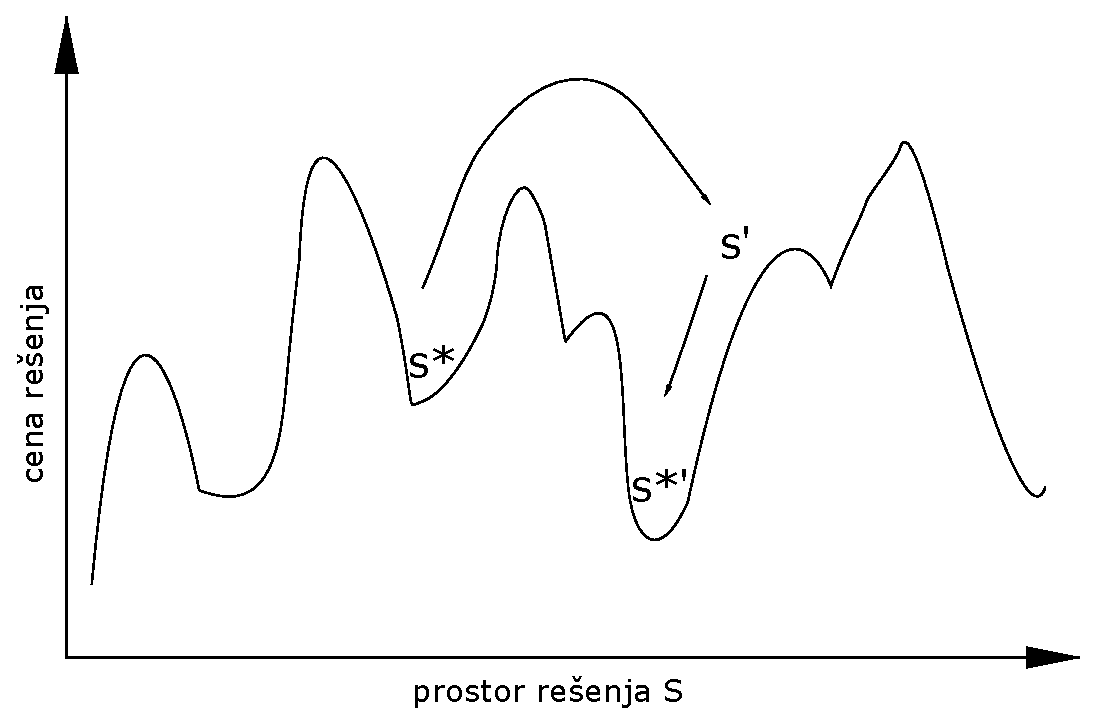
\includegraphics[width=0.8\textwidth]{drawing4.eps}
  \caption{Grafički prikaz ILS. Na trenutno rešenje \sstar{} primenjujemo \perturbacija{}, dobijamo \squote{} na koje primenjujemo \lokalna{} nakon čega dobijamo novo rešenje $\textit{s}^{*\prime{}}$.}
  \label{figure:iterativna}
\end{figure}


\begin{algorithm}
  \caption{Iterativna lokalna pretraga}
  \label{alg:1}
  \begin{algorithmic}
  \STATE $\textit{s}_0$ = \generisi{}()
  \STATE \sstar{} = \lokalna{}($\textit{s}_0$)
  \REPEAT
  \STATE \squote{} = \perturbacija{}(\sstar{}, \textit{istorija})
  \STATE $\textit{s}^{*\prime}$ = \lokalna{}(\squote{})
  \STATE \sstar{} = \kriterijum{}(\sstar{}, $\textit{s}^{*\prime}$, \textit{istorija})
  \UNTIL \textsc{nije zadovoljen uslov zaustavljanja}
  \RETURN \textsc{najbolje rešenje}
  \end{algorithmic}
  \end{algorithm}

\section{Implementacija iterativne lokalne pretrage}
Kao što možemo da vidimo iz prethodnog, da bismo implementirali algoritam tj. iterativnu lokalnu pretragu, 
potrebno je da implementiramo četiri komponente: \generisi{}, \lokalna{}, \perturbacija{} i \kriterijum{}. 

\subsection{Početno rešenje}

Početno rešenje može biti veoma važno, pogotovo ako nam je cilj što brži dolazak do kvalitetnih rešenja. 
Generisanje početnih rešenja se može izvesti na dva načina. Možemo da koristimo (\romannumeral 1) metodu slučajnog izbora, 
ili (\romannumeral 2) metodu pohlepne heuristike. U opštem slučaju, nije moguće reći koji metod od ova dva je bolji. Ipak, za kraća 
izvršavanja ILS preporučuje se metoda pohlepne heuristike, dok prilikom dužeg izvršavanja ILS izbor početnog rešenja nije mnogo bitan \cite{beginnersIntroduction}.

\subsection{Perturbacija}

Perturbacije odnosno pomeranja su veoma važna komponenta ovog algoritma. Naime, one služe da se pobegne od lokalnih minimuma (optimalnih rešenja) koji su često 
znatno lošiji od globalnog minimuma. ILS to čini tako što primenjuje perturbaciju na trenutni lokalni minimum. Definisaćemo snagu odnosno intenzitet perturbacije 
kao broj komponenti rešenja koji je perturbacijom promenjen. Snaga perturbacije je osobina koja najviše utiče na ovu komponentu algoritma. Naime, ako je snaga previše velika 
onda će se algoritam ponašati kao prilikom pokretanja lokalne pretrage iz nasumičnih delova prostora pretrage, a ako je previše mala, lokalna pretraga će često 
poništiti perturbaciju i kao novo rešenje 
naći ono od koga je krenula. Samim tim malo novih rešenja će biti istraženo. Ova veličina varira od problema do problema, a takođe zavisi i od veličine problema. 
Ponašanje ILS u praksi pokazuje da ne postoji jedinstvena optimalna snaga perturbacije. Ona se može menjati tokom izvršavanja i tada koristimo adaptivne perturbacije. 
Jedan način da se one implementiraju jeste korišćenjem istorije pretrage. Drugi način jeste determinističkim određivanjem tokom izvršavanja.

\subsection{Kriterijum prihvatanja}

Nakon što dobijemo novo moguće rešenje $\textit{s}^{*\prime}$, na osnovu procedure \kriterijum{} odlučujemo da li to rešenje prihvatamo kao novo trenutno rešenje. 
Možemo imati neki od dva ekstremna pristupa:
\begin{itemize}
  \item Uvek prihvatamo novo rešenje
  \item Ako je novo rešenje $\textit{s}^{*\prime}$ bolje od \sstar{}, onda ga prihvatamo, inače ne
\end{itemize}
Mnogi pristupi između ova dva su svakako mogući i često korišćeni. \\
\kriterijum{} ima jak uticaj na prirodu korišćenih rešenja. Naime, u kombinaciji sa \perturbacija{}, može da se 
koristi za kontrolu ravnoteže izmedju intenzifikacije\footnote{Prihvatanjem samo boljih rešenja, smanjićemo prostor pretrage i pretraživati rešenja u trenutnoj okolini} \eng{intensification} 
i diverzifikacije\footnote{Prihvatanjem svih rešenja, povećavamo prostor pretrage i imamo veliki broj rešenja, ali često pretražujemo okoline sa lošim rešenjima} \eng{diversification}. Kao i kod perturbacije 
možemo koristiti istoriju pretrage za dinamičko određivanje kriterijuma prihvatanja.

\subsection{Lokalna pretraga}

Do sada smo lokalnu pretragu koju koristi ILS koristili kao crnu kutiju \eng{black box}. Znali smo šta ta procedura radi ali nismo ulazili u detalje implementacije. Ipak, često nam je implementacija lokalne pretrage poznata 
i to nam omogućava da dodatno optimizujemo ILS. Postoji mnogo algoritama koji mogu da se koriste kao lokalna pretraga. Može se pretpostaviti da što je bolja lokalna pretraga to je bolji ILS. To često jeste tačno ali postoje 
situacije kada lošiji algoritam daje bolja rešenja. Jedna od tih situacije je kada imamo ograničeno vreme izvršavanja programa i tada je nekad bolje koristiti brži, u teoriji lošiji algoritam i pozvati ga mnogo više puta nego 
bolji i sporiji algoritam. Zavisno od razlike u potrebnom vremenu, možemo dozvoliti više vremena za izvršavanje i koristiti bolji algoritam. Ako razlika u brzini dva algoritma nije velika, onda je obično isplativije koristiti bolji. 
Za određene probleme, često se kao lokalna pretraga koristi metaheuristika poput tabu pretrage \eng{tabu search}, simuliranog kaljenja \eng{simulated annealing} itd \cite{handbookOfMetaheuristics}.

%%%%%%%%%%%%%%%%%%%%%%%%%%%%%%%%%%%%%%%%%%%%%%%%%%%%%%%%%%%%%%%%%%%%%%%%%%%%%%%%%%%%%%%%%%%%%%%%%%%%%%%%%%%%%%%%%
%%%%%%%%%%%%%%%%%%%%%%%%%%%%%%%%%%%%%%%%%%%%%%%%%%%%%%%%%%%%%%%%%%%%%%%%%%%%%%%%%%%%%%%%%%%%%%%%%%%%%%%%%%%%%%%%%
% Kraj dela (za menjanje pitati autora ovog dela)
% autor: Lazar Perisic
%%%%%%%%%%%%%%%%%%%%%%%%%%%%%%%%%%%%%%%%%%%%%%%%%%%%%%%%%%%%%%%%%%%%%%%%%%%%%%%%%%%%%%%%%%%%%%%%%%%%%%%%%%%%%%%%%
%%%%%%%%%%%%%%%%%%%%%%%%%%%%%%%%%%%%%%%%%%%%%%%%%%%%%%%%%%%%%%%%%%%%%%%%%%%%%%%%%%%%%%%%%%%%%%%%%%%%%%%%%%%%%%%%%


\section{Zaključak}
\label{sec:zakljucak}




\addcontentsline{toc}{section}{Literatura}
\appendix
\bibliography{seminarski} 
\bibliographystyle{plain}





\end{document}
